\chapter{Traitement de texte 3}  


{\footnotesize
\begin{itemize}
\item Logiciel\footnote{Le logiciel \emph{LibreOffice} est librement téléchargeable : \url{http://www.libreoffice.org/}. La version utilisée lors de la composition de ce document est la 5.1.} : \emph{LibreOffice Writer} 
\item Matières concernées : anglais, mathématiques, français.
\item Compétences : 
        \begin{itemize}
        \item gestion des styles ;
	\item insertion d'une table des matières ;
	\item en-tête et pied de page ;
	\item insertion d'un champ automatique (numéro de page) ;
	\item texte en exposant et en indice ;
	\item insertion de caractères spéciaux ; 
	\item écriture de formules mathématiques.
        \end{itemize}
\item Cette fiche est à réaliser :
        \begin{itemize}
        \item avant les vacances d'octobre en anglais (séance 1) ;
	\item avant les vacances de Noël en français (séance 2) ;
        \item avant les vacances de printemps en mathématiques (séance 3).
         
        \end{itemize}
\end{itemize}
}% fin du footnotesize



% \hfill 
\includegraphics[width=3cm]{./images/generales/VuEn6e}

\section*{Les années précédentes, vous avez appris...}

Les compétences listées ci-dessous ont été vues en classes de 6\up{e} et de 5\up{e}. Vous en aurez à nouveau besoin pour les activités de cette année. Si nécessaire, reportez-vous aux \emph{Fiches MITIC} des années précédentes pour revoir comment :  

\begin{itemize}
\item mettre en forme la page (6\up{e}) ;
\item mettre en forme des caractères (police, italique, gras, souligné, couleur) (6\up{e}) ;
\item mettre en forme des paragraphes (aligner à gauche ou à droite, justifier, retraits et espacements autour du paragraphe, encadrement) (6\up{e}) ;
\item insérer une image dans un texte (retailler l'image, conserver le ratio) (6\up{e}) ;
\item exporter un document au format PDF (6\up{e}) ;
\item insérer un tableau et définir ses propriétés (5\up{e}) ;
\item insérer une liste à puces (5\up{e}) ;
\item insérer un lien hypertexte vers un site internet (5\up{e}) ;
\item utiliser le correcteur d'orthographe (5\up{e}) ;
\item insérer une image et adapter le texte autour de l'image (5\up{e}).
\end{itemize}



\section{Les outils dont vous aurez besoin}\label{Texte4eOutils}

Les nouveaux outils dont vous aurez besoin pour réaliser les trois séances sur le traitement de texte sont décrits ci-dessous :

%\hfill
\includegraphics[width=4cm]{./images/generales/NouvelOutil}

\begin{itemize}   
\item gestion des styles, voir section \vref{Texte3styles} ;
\item insertion d'une table des matières, voir section \vref{Texte3tableMatiere} ;
\item en-tête et pied de page, voir section \vref{Texte3entetePied} ;
\item insertion d'un champ automatique (numéro de page), voir section \vref{Texte3champAuto} ;
\item texte en exposant et en indice, voir section \vref{Texte3exposantIndice} ;
\item insertion de caractères spéciaux, voir section \vref{Texte3caracteresSpeciaux} ; 
\item écriture de formules mathématiques, voir section \vref{Texte3formulesMaths}. 
\end{itemize}  




\subsection{La gestion des styles}\index{Writer!Les styles}\index{Styles (Writer)}\label{Texte3styles}

Un style est une mise en forme d'un texte, d'un paragraphe, d'une page, etc., destiné à être utilisé en plusieurs endroits d'un document. Gérer la mise en forme avec les styles permet de gagner du temps et d'obtenir une présentation plus homogène des documents.

Exemples :
\begin{itemize}
\item Un document contient quinze paragraphes. Pour modifier la taille ou la couleur des quinze titres de paragraphes, on peut le faire un par un mais cela est très long et il y a le risque d'en oublier un. Si on applique aux titres de paragraphe un seul et même style : \emph{«\,Titre 1\,»} par exemple, alors il suffit de modifier le style \emph{«\,Titre 1\,»} pour que tous les titres de paragraphe soient modifiés en même temps.
\item Dans un grand document, les textes importants sont en «\,gras\,». Vous souhaitez modifier ce choix et les faire apparaître en «\,italique\,». Si vous avez utilisé un style de caractère \emph{«\,Texte important\,»}, vous n'avez qu'à modifier le style pour que la modification soit appliquée à tous les textes importants.
\end{itemize}

\subsubsection{Style de paragraphe «\,Titre 1\,»}

\begin{enumerate}
\item Pour attribuer un style à un titre, positionner le curseur sur le titre en question (inutile de sélectionner du texte puisque c'est tout le titre qui va être affecté) puis : 

\begin{itemize}
\item soit cliquer sur le menu \texttt{Styles} puis choisir le style \texttt{Titre 1};
\item soit cliquer sur la flèche à droite de la boîte de style (voir image de droite ci-dessous) et choisir le style \texttt{Titre 1}.
\end{itemize}

\deuximagesici{./images/texte03/Texte03_Styles01}{.6\textwidth}{./images/texte03/Texte03_Styles02}{.6\textwidth}

\item Une fois que vous avez affecté le style \texttt{Titre 1} à tous les titres de paragraphe, pour changer un des attributs de mise en forme des \emph{«\,Titre 1\,»}, cliquer sur le menu \texttt{Styles} puis choisir \texttt{Éditer le style}.

\uneimageici{./images/texte03/Texte03_Styles03}{.2\textwidth}

\item Dans la fenêtre de dialogue qui s'ouvre, les onglets du haut présentent tous les attributs qui peuvent être modifiés (figure à gauche ci-dessous). Pour modifier la taille de la police, cliquer sur l'onglet \texttt{Police} puis dans le cadre \texttt{taille}. Si la taille est exprimée en pourcentage, supprimer le symbole \texttt{\%} et le remplacer par \texttt{pt} qui permet de donner la taille en points (figure à droite ci-dessous).

\deuximagesici{./images/texte03/Texte03_Styles04}{\textwidth}{./images/texte03/Texte03_Styles05&06}{\textwidth}

\item Cliquer ensuite sur l'onglet \texttt{Effets de caractères} pour modifier la couleur du texte et ajouter un soulignement.

\uneimageici{./images/texte03/Texte03_Styles07}{.5\textwidth}

\item Une fois les modifications effectuées, cliquer sur \texttt{OK} et tous les titres de paragraphe sont modifiés (figure ci-dessous).

\uneimageici{./images/texte03/Texte03_Styles08}{.7\textwidth}

\end{enumerate}


\subsection{Travailler avec les styles}\index{Writer!Travailler avec les styles}\index{Travailler avec les styles (Writer)}\label{Texte3travaillerStyle}

Trois remarques concernant le travail avec les styles :

\begin{itemize}
\vspace{8pt}\item Lorsqu'on effectue des copier/coller depuis d'autres sources (internet, autres documents, etc.), pour éviter les problèmes de formatage, le mieux est de passer par le menu \texttt{Édition}, de choisir \texttt{Collage spécial} puis \texttt{Texte non formaté}. Ainsi aucun nouveau style de paragraphe ou de caractère n'est ajouté au document en cours de travail.
\vspace{8pt}\item Il existe également des styles de caractère (par exemple un style \emph{«\,Texte important\,»} qui est affecté aux mots à mettre en valeur). Il faut savoir que les styles de caractère sont toujours prioritaires sur les styles de paragraphe.
\vspace{8pt}\item Quand on applique un style à un paragraphe, si tout ou partie du texte ne prend pas la forme voulue, deux cas peuvent se présenter :
    \begin{itemize}
    \item les caractères ont un style de caractère qui reste prioritaire ;
    \item les caractères ont été formatés sans style.
    \end{itemize}
Dans les deux cas, le plus simple consiste à effectuer un couper/collage spécial, en choisissant l'option \emph{texte non formaté}.
\end{itemize}


\subsection{Insérer une table des matières}\index{Writer!Table des matières}\index{Tables des matières (Writer)}\label{Texte3tableMatiere}

Si on utilise les styles pour les titres de paragraphes, alors on peut générer une table des matières automatique. Pour cela, positionner le curseur à l'endroit où la table doit être insérée; cliquer sur le menu \texttt{Insertion} puis sur \texttt{Table des matières et index} et enfin sur \texttt{Table des matières, index ou bibliographie…}

\uneimageici{./images/texte03/Texte03_TableMatiere1}{.5\textwidth}

Dans la fenêtre qui s'ouvre, on peut changer le nom de la table (remplacer par \emph{Sommaire} par exemple). Terminer en appuyant sur le bouton \texttt{OK}.

\uneimageici{./images/texte03/Texte03_TableMatiere2}{.7\textwidth}

\cadre{\textbf{Actualisation :} si on modifie ou rajoute des titres de chapitres, la table des matières n'est pas mise à jour automatiquement. Pour la mettre à jour, positionner la souris sur la table des matières, faire un clic droit et sélectionner \texttt{Actualiser l'index}.}


\subsection{En-tête et pied de page}\index{Writer!En-tête}\index{En-tête (Writer)}\index{Writer!Pied de page}\index{Pied de page (Writer)}\label{Texte3entetePied}

Pour ajouter un en-tête ou un pied de page, sélectionner le menu \texttt{Format} puis \texttt{Page...} Dans la fenêtre qui s'ouvre, sélectionner l'onglet \texttt{En-tête} puis cocher la case \texttt{Activer l'en-tête} et cliquer sur \texttt{OK}.

\deuximagesici{./images/texte03/Texte03_Entete1}{.5\textwidth}{./images/texte03/Texte03_Entete2}{\textwidth}

Pour remplir l'en-tête, il faut cliquer dessus avant de mettre son texte.

\uneimageici{./images/texte03/Texte03_Entete3}{.7\textwidth}

L'activation du pied de page se fait de la même manière :

\uneimageici{./images/texte03/Texte03_PieddePage1}{.5\textwidth}


\emph{Remarque :} l'en-tête et le pied de page sont définis de telle manière que l'on peut, en appuyant une fois sur la touche \texttt{Tabulation}, entrer un texte centré au milieu de la page et en appuyant une deuxième fois, entrer un texte aligné à droite de la page.



\subsection{Insérer un champ automatique (numéro de page)}\index{Writer!Champ automatique}\index{Champ automatique (Writer)}\index{Writer!Numéro de page}\index{Numéro de page (Writer)}\label{Texte3champAuto}

Dès qu'un document fait plus de quelques pages, il devient intéressant de placer dans l'en-tête ou le pied de page une numérotation automatique des pages. Pour cela, on utilise un \emph{champ automatique}. 

Par exemple, écrire le texte \emph{Page } dans le pied de page. Sélectionner le menu \texttt{Insertion} puis \texttt{Champ} puis \texttt{Numéro de page}. Le numéro de la page est automatiquement inséré à l'endroit où se trouvait le curseur.

\uneimageici{./images/texte03/Texte03_InsereChamp1}{.5\textwidth}

Ajouter une barre oblique : \emph{/} et insérer le champ automatique \texttt{Nombre de pages}.

\deuximagesici{./images/texte03/Texte03_InsereChamp2}{\textwidth}{./images/texte03/Texte03_InsereChamp3}{0.6\textwidth}

\textbf{Remarque :} à l'écran, les champs automatiques apparaissent sur un fond grisé. Ce fond est là pour repérer qu'il s'agit d'un champ automatique mais il n'est pas imprimé.



\subsection{Mettre du texte en exposant et en indice}\index{Writer!Exposant}\index{Exposant (Writer)}\index{Writer!Indice}\index{Indice (Writer)}\label{Texte3exposantIndice}

Pour mettre du texte en exposant ou en indice, il faut sélectionner le texte concerné puis cliquer sur le menu \texttt{format} puis choisir \texttt{caractère}.

\uneimageici{./images/texte03/texte3indice1}{.4\textwidth}

Dans la fenêtre de dialogue qui s'ouvre alors, choisir l'onglet \texttt{Position} puis sélectionner \texttt{exposant} ou \texttt{indice}.

\deuximagesici{./images/texte03/texte3indice2}{.95\textwidth}%
	    {./images/texte03/texte3exposant1}{.95\textwidth}

Le résultat obtenu est montré sur la figure ci-dessous.

\uneimageici{./images/texte03/texte3exposantResultat}{.4\textwidth}

Pour mettre le texte en exposant ou en indice, il également possible, après avoir sélectionné le texte, de :
\begin{itemize}
\item cliquer directement sur les icônes correspondantes pour mettre du texte en indice 
\includegraphics[width=.6cm]{./images/texte03/texte3indiceIcone} ou en exposant 
\includegraphics[width=.6cm]{./images/texte03/texte3exposantIcone} ;
\item utiliser le raccourci clavier \texttt{Cmd + Shift + B} pour mettre le texte en indice (\emph{B} pour \emph{Bottom}) et \texttt{Cmd + Shift + P} pour mettre le texte en exposant (\emph{P} pour \emph{Power}). 
\end{itemize}


\subsection{Insérer des caractères spéciaux}\index{Writer!Caractères spéciaux}\index{Caractères spéciaux (Writer)}\label{Texte3caracteresSpeciaux}

Pour écrire un caractère qui n'est pas accessible directement sur les touches du clavier, comme par exemple des lettres grecques souvent utilisées dans les sciences, positionner le curseur à l'endroit où on souhaite l'insérer, cliquer sur le menu \texttt{Insertion} et choisir \texttt{caractères spéciaux…}

\uneimageici{./images/texte03/texte3caracteresSpe1}{.5\textwidth}

Dans la boîte de dialogue qui s'ouvre (figure ci-dessous), il faut :
\begin{itemize}
\item \circled{1} sélectionner la police (chaque police propose des caractères spéciaux qui lui sont propres ; si on ne trouve pas le caractère cherché dans une police, on peut en essayer une autre);
\item \circled{2} éventuellement changer le sous-ensemble de caractères;
\item \circled{3} sélectionner le caractère cherché ;
\item \circled{4} appuyer sur le bouton \texttt{Insérer} pour terminer.
\end{itemize}

\uneimageici{./images/texte03/texte3caracteresSpe2}{.7\textwidth}



\subsection{Écrire des formules mathématiques}\index{Writer!Formules mathématiques}\index{Formules mathématiques (Writer)}\label{Texte3formulesMaths}

\emph{LibreOffice Writer} propose un éditeur de formules mathématiques qui permet de mettre en forme les fractions, les racines carrées, les systèmes, etc.

Pour insérer une formule mathématique, cliquer sur le menu \texttt{Insertion} puis choisir \texttt{Objet} et enfin \texttt{Formule...}


\uneimageici{./images/texte03/Texte03_Formule1}{.4\textwidth}

Une fenêtre s'ouvre alors. Elle permet de visualiser plusieurs parties (figure ci-dessous) :
\begin{itemize}
\item \circled{1} la formule telle qu'elle va apparaître dans le document;
\item \circled{2} le texte de la formule dans l'éditeur de formule;
\item \circled{3} une fenêtre d'aide à la mise en forme des formules.
\end{itemize}

\uneimageici{./images/texte03/Texte03_Formule2}{.8\textwidth}

Dans la fenêtre d'aide à la mise en forme, on sélectionne un type de formule (parcourir les différents items pour voir les propositions).

\uneimageici{./images/texte03/Texte03_Formule3}{.4\textwidth}

Pour écrire une fraction, on choisit le type \texttt{Opérateurs unaires/binaires} et on sélectionne le modèle 
\includegraphics[width=.6cm]{./images/texte03/Texte03_Formule7} (\circled{1} sur la figure ci-dessous à gauche). La fenêtre de formule affiche 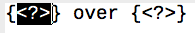
\includegraphics[width=3cm]{./images/texte03/Texte03_Formule8} (\circled{2}) et il suffit alors de remplir chacun des champs de la forme \texttt{<?>} (\circled{3}), par exemple avec 1 et 2.

\deuximagesici{./images/texte03/Texte03_Formule4}{\textwidth}{./images/texte03/Texte03_Formule9}{0.5\textwidth}

\emph{Remarque :} Pour sortir du mode écriture de formule et revenir au document, il suffit de cliquer une fois dans la fenêtre du document. Pour modifier une formule existante, double-cliquer dessus et la fenêtre de l'éditeur de formule s'ouvre.

On peut aussi entrer du texte dans une formule. Dans l'exemple suivant, on a ajouté \texttt{cosinus =} avant les champs \texttt{<?>} puis entré les textes \texttt{côté opposé} et \texttt{hypothénuse} dans la fraction. Dans ce cas, on remarque que les textes apparaissent en italique dans le document : par défaut le texte entré dans une formule est considéré comme une variable mathématique. Si on veut éviter cela, on entoure le texte de guillemets (image de droite ci-dessous).

\deuximagesici{./images/texte03/Texte03_Formule5}{.9\textwidth}{./images/texte03/Texte03_Formule6}{\textwidth}





%
%
%  S  É  A  N  C  E     I
%
%

\pagebreak

\section{Séance 1 : un exposé sur un pays (anglais)}\label{ficheTexte4e2}


\boiteEnonceLarge{Le but de cette séance est de rédiger un exposé en anglais sur un pays de votre choix à l'aide du traitement de texte \emph{LibreOffice Writer}.

L'exposé doit contenir les parties suivantes : 
\emph{\begin{enumerate}
\item Geography, demography, climate, main cities
\item Symbols and motto
\item Culture and tradition
\item Political regime
\item Sports
\item Famous people
\item Why did I choose this country?
\end{enumerate}
} % fin du emph

Pour cela, vous devrez :
\begin{itemize}
\item sauvegarder le fichier en le nommant à partir de votre nom : \texttt{Nom-Prénom-date.odt} ; 
\item mettre en forme la page selon vos souhaits (orientation de la page, taille des différentes marges, etc.) ; 
\item utiliser des styles pour mettre en forme les différents titres et parties ;
\item insérer au moins deux images et adapter le texte autour des images ;
\item utiliser au moins une liste à puces ; 
\item citer vos sources sous forme de notes de bas de page (ne pas oublier la source de l'image) ; 
\item insérer un en-tête qui contient votre prénom, votre nom et la date du jour ;
\item insérer un pied de page qui contient le numéro de la page et le nombre total de pages en utilisant les champs automatiques (par ex. \emph{«\,Page 1/3\,»}) ;
\item insérer au début du document une table des matières construite automatiquement.
\end{itemize}
Une fois votre travail terminé, rendre le fichier au format ODT sur la plateforme \emph{Moodle} à l'endroit indiqué par votre enseignant (si nécessaire, se reporter à la fiche méthode \emph{Remettre un devoir sur Moodle}, section \vref{MoodleRendreDevoir}).
}% fin de l'énoncé




\vfill

\cadre{Pensez à sauver régulièrement votre travail en appuyant sur \texttt{Cmd + S} ou à partir du menu \texttt{Fichier} en choisissant \texttt{Enregistrer}.

\uneimageici{./images/generales/clavierCmdS}{.3\textwidth}
}


%
%
%  S  É  A  N  C  E     II
%
%

\pagebreak

\section{Séance 2 : une fiche de lecture (français)}\label{ficheTexte4e3}



\boiteEnonceLarge{Le but de cette séance est de mettre en forme une fiche de lecture à l'aide du traitement de texte \emph{LibreOffice Writer}. La structure de la fiche de lecture vous sera communiquée par votre enseignant de français. 

Pour cela, vous devrez :
\begin{itemize}
\item sauvegarder le fichier en le nommant à partir de votre nom : \texttt{Nom-Prénom-date.odt} ; 
\item mettre en forme la page selon vos souhaits (orientation de la page, taille des différentes marges, etc.) ; 
\item utiliser des styles pour mettre en forme les différents titres et parties ;
\item insérer au moins une image et adapter le texte autour des images ;
\item utiliser au moins une liste à puces ; 
\item citer vos sources sous forme de notes de bas de page (ne pas oublier la source de l'image) ; 
\item insérer un en-tête qui contient votre prénom, votre nom et la date du jour ;
\item insérer un pied de page qui contient le numéro de la page et le nombre total de pages en utilisant les champs automatiques (par ex. \emph{«\,Page 1/3\,»}) ;
\item insérer au début du document une table des matières construite automatiquement.
\end{itemize}
Une fois votre travail terminé, rendre le fichier au format ODT sur la plateforme \emph{Moodle} à l'endroit indiqué par votre enseignant (si nécessaire, se reporter à la fiche méthode \emph{Remettre un devoir sur Moodle}, section \vref{MoodleRendreDevoir}).


}% fin énoncé

\vfill

\cadre{Pensez à sauver régulièrement votre travail en appuyant sur \texttt{Cmd + S} ou à partir du menu \texttt{Fichier} en choisissant \texttt{Enregistrer}.

\uneimageici{./images/generales/clavierCmdS}{.3\textwidth}
}


%
%
%  S  É  A  N  C  E     III
%
%




\pagebreak

\section{Séance 3 : correction d'exercices sur les fonctions}\label{ficheTexte4e1}

\boiteEnonceLarge{Le but de cette séance est de rédiger la correction d'un ou plusieurs exercices de mathématiques à l'aide du traitement de texte \emph{LibreOffice Writer}. Pour cela, vous devrez :
\begin{itemize}
\item sauvegarder le fichier en le nommant à partir de votre nom : \texttt{Nom-Prénom-date.odt} ; 
\item utiliser des styles pour mettre en forme les titres de chaque exercice ;
\item utiliser des listes numérotées pour répondre aux différentes questions de chaque exercice ; 
\item utiliser l'outil d'écriture de formules mathématiques pour les parties mathématiques ;
\item insérer un en-tête qui contient votre prénom, votre nom et la date du jour ;
\item insérer un pied de page qui contient le numéro de la page et le nombre total de pages en utilisant les champs automatiques (par ex. \emph{«\,Page 1/3\,»}) ;
\item insérer au début du document une table des matières construite automatiquement.
\end{itemize}
Une fois votre travail terminé, rendre le fichier au format ODT sur la plateforme \emph{Moodle} à l'endroit indiqué par votre enseignant (si nécessaire, se reporter à la fiche méthode \emph{Remettre un devoir sur Moodle}, section \vref{MoodleRendreDevoir}).
}% fin de l'énoncé

\vfill

\cadre{Pensez à sauver régulièrement votre travail en appuyant sur \texttt{Cmd + S} ou à partir du menu \texttt{Fichier} en choisissant \texttt{Enregistrer}.

\uneimageici{./images/generales/clavierCmdS}{.3\textwidth}
}



